\documentclass{article}
\usepackage{graphicx}
\usepackage{geometry}
\usepackage{listings}
\geometry{a4paper, margin=1in}

\title{Statistiques du Jeu}

\begin{document}
\maketitle

\section*{Temps moyen de réaction par joueur}
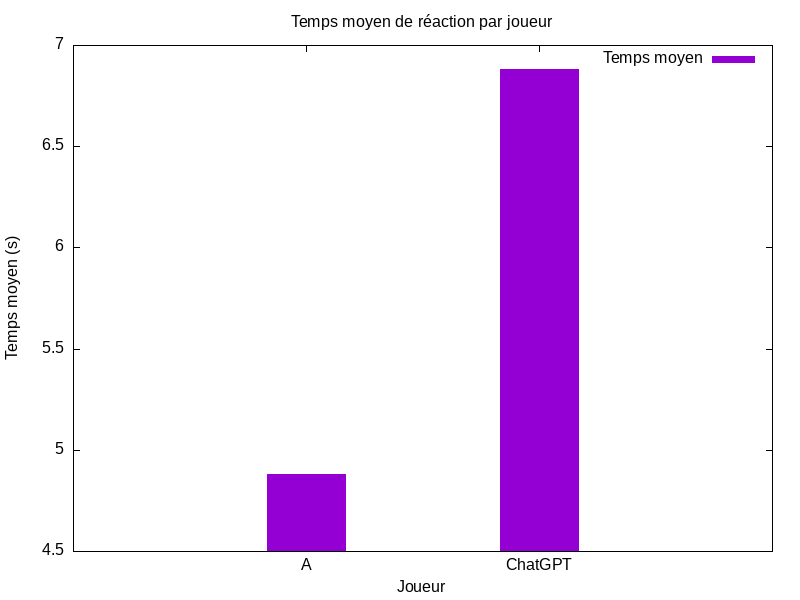
\includegraphics[width=\textwidth]{../Graphiques/temps_reaction_par_joueur.png}

\section*{Histogramme des valeurs ayant causé l'échec}
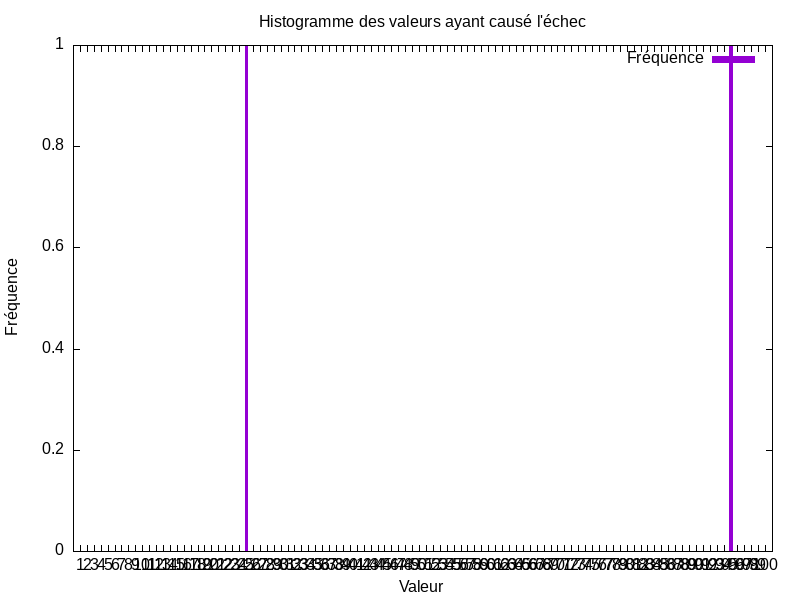
\includegraphics[width=\textwidth]{../Graphiques/valeurs_echec.png}

\section*{Manches réussies par joueur}
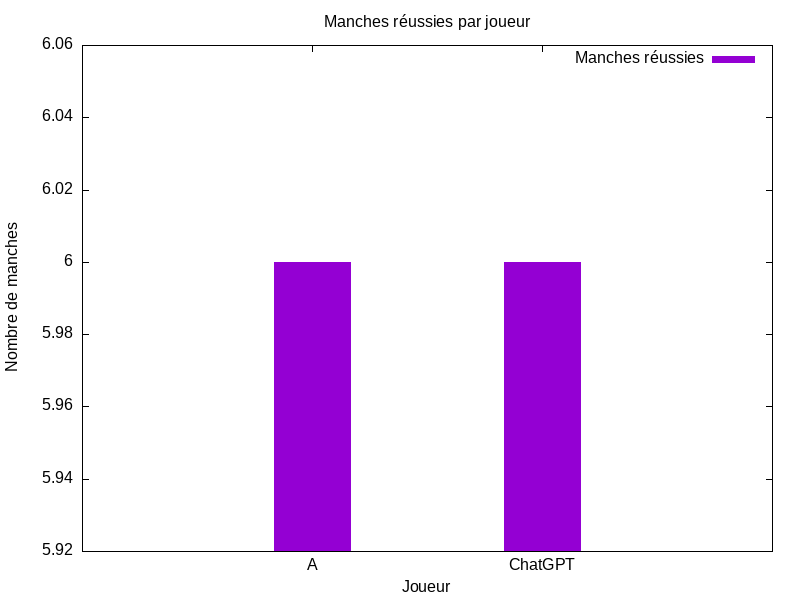
\includegraphics[width=\textwidth]{../Graphiques/manches_reussies_par_joueur.png}

\section*{Classement des joueurs}
\lstinputlisting{../classement_joueurs.txt}

\end{document}